%%%%%%%%%%%%%%%%%%%%%%%%%%%%%%%%%%%%%%%%%
% Beamer Presentation
% LaTeX Template
% Version 1.0 (10/11/12)
%
% This template has been downloaded from:
% http://www.LaTeXTemplates.com
%
% License:
% CC BY-NC-SA 3.0 (http://creativecommons.org/licenses/by-nc-sa/3.0/)
%
%%%%%%%%%%%%%%%%%%%%%%%%%%%%%%%%%%%%%%%%%

%----------------------------------------------------------------------------------------
%	PACKAGES AND THEMES
%----------------------------------------------------------------------------------------
\PassOptionsToPackage{dvipsnames}{xcolor}

\documentclass[xcolor=dvipsnames]{beamer}

\mode<presentation> {

% The Beamer class comes with a number of default slide themes
% which change the colors and layouts of slides. Below this is a list
% of all the themes, uncomment each in turn to see what they look like.

%\usetheme{default}
%\usetheme{AnnArbor}
%\usetheme{Antibes}
%\usetheme{Bergen}
%\usetheme{Berkeley}
%\usetheme{Berlin}
%\usetheme{Boadilla}
%\usetheme{CambridgeUS}
%\usetheme{Copenhagen}
%\usetheme{Darmstadt}
%\usetheme{Dresden}
%\usetheme{Frankfurt}
%\usetheme{Goettingen}
%\usetheme{Hannover}
%\usetheme{Ilmenau}
%\usetheme{JuanLesPins}
%\usetheme{Luebeck}
\usetheme{Madrid}
%\usetheme{Malmoe}
%\usetheme{Marburg}
%\usetheme{Montpellier}
%\usetheme{PaloAlto}
%\usetheme{Pittsburgh}
%\usetheme{Rochester}
%\usetheme{Singapore}
%\usetheme{Szeged}
%\usetheme{Warsaw}

% As well as themes, the Beamer class has a number of color themes
% for any slide theme. Uncomment each of these in turn to see how it
% changes the colors of your current slide theme.

%\usecolortheme{albatross}
%\usecolortheme{beaver}
%\usecolortheme{beetle}
%\usecolortheme{crane}
\usecolortheme{dolphin}
%\usecolortheme{dove}
%\usecolortheme{fly}
%\usecolortheme{lily}
%\usecolortheme{orchid}
%\usecolortheme{rose}
%\usecolortheme{seagull}
%\usecolortheme{seahorse}
%\usecolortheme{whale}
%\usecolortheme{wolverine}

%\setbeamertemplate{footline} % To remove the footer line in all slides uncomment this line
%\setbeamertemplate{footline}[page number] % To replace the footer line in all slides with a simple slide count uncomment this line

\setbeamertemplate{navigation symbols}{} % To remove the navigation symbols from the bottom of all slides uncomment this line
}



\input inputs/packages.tex
\input inputs/abbreviations.tex
\input inputs/commands.tex

%----------------------------------------------------------------------------------------
%	TITLE PAGE
%----------------------------------------------------------------------------------------

\newcommand\meeting{Thesis defense}

\title[\meeting]{Measurement of the photon energy spectrum in
inclusive radiative \texorpdfstring{$B$}{B} meson decays using the
hadronic-tagging method} % The short title appears at the bottom of every slide, the full title is only on the title page

\author[Henrikas Svidras]{\texorpdfstring{\footnotesize \underline{Henrikas Svidras}}{Henrikas Svidras}} % Your name
%\subject{\text{\small KEK, Tsukuba}}
\institute[DESY] % Your institution as it will appear on the bottom of every slide, may be shorthand to save space
{
\text{\large \meeting}
\vspace{-10pt}
}
\titlegraphic{
\includegraphics[width=2cm]{logos/DESY.png}\hspace*{4.75cm}~%
   
\includegraphics[width=2cm]{logos/belle2.png}
}

\date{March 13, 2023} % Date, can be changed to a custom date

\begin{document}

\setbeamercolor{background canvas}{bg=}
{\setbeamertemplate{footline}{} 
\begin{frame}
\titlepage % Print the title page as the first slide
\end{frame}
}
\addtocounter{framenumber}{-1}


%----------------------------------------------------------------------------------------
%	INTRO
%----------------------------------------------------------------------------------------
\section{Introduction}

\begin{frame}

   \centering

{\LARGE Measurement of the photon energy spectrum in
{\color{OrangeRed}inclusive} {\color{YellowGreen}radiative} \texorpdfstring{$B$}{B} meson decays using the
{\color{MidnightBlue}hadronic-tagging} method}

\vspace{10pt}

\textbf{Let's look at these three terms closer}

\end{frame}

\begin{frame}{Introduction: radiative \safeB meson decays}
\centering\scriptsize
{\normalsize What are \textbf{radiative $\bm{B}$} decays?
\begin{columns}
   \column{0.4\textwidth}
   \begin{tikzpicture}
    \begin{feynman}
    \vertex (i1){b};
    \vertex[right =1.2cm of i1] (a);
    \vertex[right=0.85cm of a] (b);
    \vertex[right=0.85cm of b] (c);
    \vertex[right=1.2cm of c] (o1) {s,d};
    \vertex[below=2em of c] (g1);
    \vertex[right=2em of g1] (o2) {$\gamma$};
    
    \diagram* {
    (i1) -- [fermion] (a) -- [fermion, edge label =\(uct\)] (c) -- [fermion] (o1),
    (a) -- [boson,half left, edge label = \(W^{\pm}\)] (c),
    (b) -- [photon] (o2),
    };
    \end{feynman}
\end{tikzpicture}
    
   \column{0.4\textwidth}
   \begin{tikzpicture}
    \begin{feynman}
    \vertex (i1){b};
    \vertex[right =1.2cm of i1] (a) ;
    \vertex[right=0.85cm of a] (b);
    \vertex[right=0.85cm of b] (c);
    \vertex[right=1.2cm of c] (o1) {s,d};
    \vertex[below=2em of c] (g1);
    \vertex[right=2em of g1] (o2) {$\gamma$};
    
    \diagram* {
    (i1) -- [fermion] (a) -- [boson, edge label =\(W^{\pm}\)] (c) -- [fermion] (o1),
    (a) -- [fermion,half left, edge label = \(uct\)] (c),
    (b) -- [photon] (o2),
    };
    \end{feynman}
\end{tikzpicture}
    
\end{columns}
}

\begin{itemize}
   \item Rare decays: \textbf{forbidden at tree level} in the Standard Model!
   \item \textbf{New particles} can appear \textbf{in the loops}, one of many examples:
\end{itemize}
{\normalsize
\begin{columns}
   \column{0.4\textwidth}
   \begin{tikzpicture}
    \begin{feynman}
    \vertex (i1){b};
    \vertex[right =1.2cm of i1] (a) ;
    \vertex[right=0.85cm of a] (b);
    \vertex[right=0.85cm of b] (c);
    \vertex[right=1.2cm of c] (o1) {s,d};
    \vertex[below=2em of c] (g1);
    \vertex[right=2em of g1] (o2) {$\gamma$};
    
    \diagram* {
    (i1) -- [fermion] (a) -- [scalar, edge label =\(H^{\pm}\)] (c) -- [fermion] (o1),
    (a) -- [fermion,half left, edge label = \(uct\)] (c),
    (b) -- [photon] (o2),
    };
    \end{feynman}
\end{tikzpicture}
\end{columns}
}
\begin{itemize}
   \item In the case of \btosgamma: $\mathcal{B}\sim10^{-4}$.
   \item[\ra] Accessible with smaller datasets than e.g. $b\to s\ell\ell$, where $\mathcal{B}\sim10^{-6}$
\end{itemize}

\end{frame}

\begin{frame}{Introduction: inclusive \safeB meson decays}
   \centering\scriptsize
   {\normalsize What are \textbf{inclusive $\bm{B}$} decays?}

   \vspace{10pt}

   \begin{itemize}
      \item $B$ mesons are the \textbf{lightest mesons involving a $\bm{b}$ quark}
      \item[\ra] decays always involve one or more flavour/generation changes!
      \item[\ra] plethora of final decay states from $u, d, c, s$ quarks
   \end{itemize}

   \vspace{10pt}

   \begin{columns}
      \column{0.5\textwidth}
      \centering
         \textbf{Exclusive}: pick a particular state and study its properties
            \begin{itemize}
               \item $B^0\to{K^0}^*(892)\gamma$
               \item $B^+\to K^+\mu^+\mu^-$
            \end{itemize}
      \column{0.5\textwidth}
      \centering
         \textbf{Inclusive}: study all states originating from the associated quark
         \begin{itemize}
            \item $B\to X_s \gamma$
            \item $B\to X_u \ell \nu$
         \end{itemize}
   \end{columns}
   
   \vspace{10pt}
   Just a couple from many of potential examples!

\end{frame}

\begin{frame}{Introduction: hadronic tagging}
\centering\scriptsize
{\normalsize What is \textbf{hadronic tagging}?}

\vspace{10pt}

\begin{columns}
   \column{0.33\textwidth}
   \input tikz/tagging.tex

   \column{0.66\textwidth}
   \begin{itemize}
      \item Method for $\boldsymbol{e^+}\boldsymbol{e^-}$ \textbf{colliders only}!
      \item Use the known initial state of the \epem collision
      \item \textit{Tag} the signal side
      \item[\ra] the four-momentum constraint allows to \textbf{infer the charge, flavour, four-momentum} of the signal side
   \end{itemize}
\end{columns}


\end{frame}

%----------------------------------------------------------------------------------------
%	THEORY
%----------------------------------------------------------------------------------------

\section{\safeBtoXsgamma theory}

\begin{frame}{Description of the inclusive \BtoXsgamma decays}
   \scriptsize
      \begin{equation}\nonumber
         \mathcal{L}_{\mathrm{eff}} = \frac{4G_F}{\sqrt{2}}V_{tq}^*V_{tb}\left[\sum^{8}_{i=1}\mathcal{C}_i(\mu)\mathcal{O}_i(\mu)
                                                     + \cancel{\frac{V^*_{uq}V_{ub}}{V^*_{tq}V_{tb}}\sum^{2}_{i=1}\mathcal{C}_i(\mu)(\mathcal{O}_i(\mu)-\mathcal{O}_i^u(\mu))}\right]
      \end{equation}
   
   \begin{itemize}
      \item For \btosgamma the second term is much less important
      \item It is relevant for higher order corrections, and for \btodgamma
      \item[\ra] Then the effective Lagrangian takes the form:
   \end{itemize}
   
   \vspace{-0pt}
   
   \begin{equation*}
    \mathcal{L}_{\mathrm{eff}} \propto
\mathcal{C}_7 \times
\Biggl[
\raisebox{5pt}{
\resizebox{0.085\textwidth}{!}{
\feynmandiagram [small, inline=(b.base), vertical=b to d] {
    a --  b [dot] -- c,
    b -- [boson] d [particle={\LARGE$\gamma$}],
    };
}
}\Biggr]
+
\mathcal{C}_8 \times
\Biggl[
\raisebox{5pt}{
\resizebox{0.085\textwidth}{!}{
\feynmandiagram [small, inline=(b.base), vertical=b to d] {
    a --  b [dot] --  c,
    b -- [boson] d [particle={\LARGE$g$}],
    };
}
}\Biggr]
+
\sum_i^{1,...,6}
\mathcal{C}_i\times
\Biggl[
\raisebox{3pt}{
\resizebox{0.085\textwidth}{!}{
\feynmandiagram [small, inline=(b.base), horizontal=a to c] {
    a --  b [dot] --  c,
    d --  b -- e,
    };
}
}\Biggr]
+\mathrm{corrections}
\end{equation*}
   
   \begin{itemize}
      \item[\ra] massive non-Standard Model particles modify $\mathcal{C}_i$ (normalisation)
      \item[\ra] BSM probe: $      \mathcal{C}_i^{\mathrm{SM}} \ra \mathcal{C}_i^{\mathrm{SM}} + \Delta\mathcal{C}_i^{\mathrm{BSM}}$
      \item and one evaluates the decay rate as 
   \end{itemize}
   
   \vspace{-10pt}
   
   
   \begin{equation}\nonumber
      \Gamma(\btosgamma)\propto|\mel**{s\gamma}{\mathcal{L}_{\mathrm{eff}}}{b}|^2
   \end{equation}   

   \begin{equation}\nonumber
      \Gamma(B\ra\X_s\g) = \Gamma(b\ra s\g) + \underbrace{\Delta\Gamma_{\text{non-peturbative}}}_{\substack{\text{depends on}\\ \text{\Egamma (or }M_X\text{)!}}}
  \end{equation}

  \begin{itemize}
   \item theory calculations often use $\Egamma > 1.6~\gev$  which yields $\Delta\Gamma_{\text{non-peturbative}} \sim \mathcal{O}(3\%)$
  \end{itemize}
  
\end{frame}

\begin{frame}{Description of \BtoXsgamma photon energy spectrum}

   \scriptsize\centering

   Non-perturbative effects more complicated if the partial decay rates are considered

   \vspace{10pt}

   \begin{columns}
      \column{0.5\textwidth}
      \centering
      \includegraphics[width=0.8\textwidth]{../phd_thesis/figures/theory/xsgamma_theory_to_experiment.png}
      \column{0.5\textwidth}
      \centering
      \includegraphics[width=0.8\textwidth]{../phd_thesis/figures/theory/xsgamma_theory_components.png}
   \end{columns}

   \begin{itemize}
      \item $b$ quark is not stationary in the $B$ meson!
      \item such non-perturbative effects encoded in a so-called \textbf{shape-function} $\bm{\mathcal{F}}$!
      \item[\ra] it is a universal property of the $B$ meson
      \item[\ra] $\mathcal{F}$ is necessary in other analyses such as $V_{ub}$ determination from $B\to X_u\ell\nu$ 
   \end{itemize}
   
\end{frame}

   %----------------------------------------------------------------------------------------
   %	Experimental status
   %----------------------------------------------------------------------------------------
   \section{\safeBtoXsdgamma experimental status}

   \begin{frame}{\safeBtoXsgamma experimental status}
      \scriptsize
      \begin{equation}\nonumber
         \mathcal{B}(\BtoXsgamma) = (3.40\pm 0.17) \cdot 10 ^{-4}
      \end{equation}

      whereas the experimental value is:

      \begin{equation}\nonumber
         \mathcal{B}(\BtoXsgamma) = (3.49\pm 0.19) \cdot 10 ^{-4}
      \end{equation}

      which is a combination of the following measurements:
      \vspace{5pt}

      \resizebox{1.\textwidth}{!}{
         \begin{tabular}{|lllllc|}
         \hline
         Year & Experiment                 & Technique & Data used  & Energy threshold &  $\mathcal{B}(B\rightarrow X_s\gamma) \times 10^{-4}$  [$\EB>1.6~\gev$]\\ 
         \hline
         2001 & CLEO   & Untagged         & 9.1~\invfb &  $\EB>2.0~\gev$ & $3.29\pm0.44\pm0.29$\\ 
         2007 & BaBar & Hadronic-tagged  & 210~\invfb &  $\EB>1.9~\gev$ & $3.90\pm0.91\pm0.64$\\ 
         2009 & Belle & Untagged/Lepton-tagged      & 605~\invfb &  $\EB>1.7~\gev$ & $3.47\pm0.15\pm0.40$\\ 
         2012 & BaBar  & Lepton-tagged         & 347~\invfb &  $\EB>1.7~\gev$ & $3.32\pm0.16\pm0.31$\\ 
         2012 & BaBar  & Sum-of-exclusive & 429~\invfb &  $\EB>1.7~\gev$ & $3.52\pm0.20\pm0.51$\\ 
         2014 & Belle & Sum-of-exclusive & 711~\invfb &  $\EB>1.7~\gev$ & $3.75\pm0.18\pm0.35$\\
         %\hline
         %2022 & {\bf Belle II}& Hadronic               & 189 fb$^{-1}$ & $3.54 \pm0.78 (\mathrm{stat.})\pm0.83(\mathrm{syst.})$ &              $E^B_{\gamma}>1.8~\gev$                 \\
         \hline
         \end{tabular}
         }
         
         \vspace{10pt}

         Notice three prevalent type of measurement techniques:
         \begin{itemize}
            \item Sum-of-exclusive
            \item Untagged
            \item Tagged
         \end{itemize}
         \textbf{Only obtained by $\bm{B}$ factories}!
   \end{frame}

   
      \begin{frame}{\safeBtoXsgamma measurement techniques}
      \scriptsize
      \begin{columns}
         \centering
         \column{0.4\textwidth}
         \pgfdeclarelayer{bg}    % declare background layer
\pgfsetlayers{bg,main}  % set the order of the layers (main is the standard layer)
\begin{tikzpicture}[rotate=90]

    % NODES
    
    % Initial state
    \node [circle, minimum size=1.2cm, draw=white, ultra thick]    (collision) {} ;
    % \node [] (collision) {} ;
    \node [] (collisiontext) [below=0.03cm of collision.west] {\FourS};
    \node [] (eminus)     [left=2cm of collision.center] {};
    \node [] (eplus)     [right=1.5cm of collision.center] {};
    \node [] (eplusabove) [above=0.1cm of eplus] {};
    \node [] (eminusabove) [above=0.1cm of eminus] {};
    \node [] (eminustext)     [right=0.3cm of eminusabove, text=blue] {\en};
    \node [] (eplustext)     [left=0.3cm of eplusabove, text=red] {\ep};
    
    % BB bar
    \node [] (bbarup) [above=0.7cm of collision.north east] {};
    \node [] (bbardown) [below=0.5cm of collision.south east] {};
    \node [] (bbarup_text) [right=0.05cm of bbarup.center] {$\B_{\mathrm{sig}}$};
    \node [] (bbardown_text) [right=0.05cm of bbardown.center] {$\B_{\mathrm{tag}}$};
    
    % Xs gamma
    %%gamma
    \node [] (gamma_int) [left=0.5cm of bbarup.center] {};
    \node [] (gamma) [above=1cm of gamma_int.center] {};
    \node [] (gammatext) [left=0.05cm of gamma.center] {$\gamma$};
    %%xs
    \node [] (Xs_int) [right=0.5cm of bbarup.center] {};
    \node [] (Xs) [above=0.5cm of Xs_int.center] {};
    \node [] (Xstext) [left=0.05cm of Xs.center] {$X_{s}$};
    %%xs daughters
    \node [] (Xsd1_int) [left=0.05cm of Xs.center] {};
    \node [] (Xsd1) [above=0.5cm of Xsd1_int.center] {};
    \node [] (Xsd2_int) [right=0.2cm of Xs.center] {};
    \node [] (Xsd2) [above=0.4cm of Xsd2_int.center] {};
    \node [] (Xsd3_int) [right=0.35cm of Xs.center] {};
    \node [] (Xsd3) [above=0.2cm of Xsd3_int.center] {};
    
    % Tag side
    
    % first generation
    \node [] (D0_int) [left=0.35cm of bbardown.center] {};
    \node [] (D0) [below=0.65cm of D0_int.center] {};
    \node [] (pi0_int) [right=0.3cm of bbardown.center] {};
    \node [] (pi0) [below=0.6cm of pi0_int.center] {};
    
    %second generation
    \node [] (Kp_int) [left=0.25cm of D0.center] {};
    \node [] (Kp) [below=0.65cm of Kp_int.center] {};
    \node [] (pim_int) [right=0.1cm of D0.center] {};
    \node [] (pim) [below=0.6cm of pim_int.center] {};

    \node [] (g1_int) [left=0.2cm of pi0.center] {};
    \node [] (g1) [below=0.65cm of g1_int.center] {};
    \node [] (g2_int) [right=0.15cm of pi0.center] {};
    \node [] (g2) [below=0.6cm of g2_int.center] {};
    
    %\node [] (hadron text) [below=0.05cm of bbardown.center] {\scriptsize hadrons};
    
    % Colored overal blocks
    
    \node [] (sigside) [above=0.8cm of bbarup] {};
    \node [] (tagside) [below=0.8cm of bbardown] {};
    \node [] (tagside_right) [right=0.2cm of tagside] {};
    
    \node [] (sigsidetext) [above=0.1cm of sigside] {\scriptsize Signal side};
    \node [] (tagsidetext) [below=0.3cm of tagside_right, text width = 2cm] {\centering\scriptsize Tag side};
    
    \begin{pgfonlayer}{bg}    % select the background layer
    \node [rectangle, fill=green!20, text width=2cm, text centered, rounded corners, minimum height=1.7cm] (Signal_Side) at (sigside) {};
    \node [rectangle, fill=blue!20, text width=2cm, text centered, rounded corners, minimum height=1.7cm] (Signal_Side) at (tagside) {};
    \end{pgfonlayer}

    

    
    % LINES
    
    % Initial state
    \draw [-Triangle, blue, thick] (eminus) -- (collision.center);
    \draw [-Triangle, red, thick] (eplus) -- (collision.center);
    
    % BB bar
    \draw[-Triangle, thick] (collision.center) -- (bbarup.center);
    \draw[-Triangle, thick] (collision.center) -- (bbardown.center);
    
    % Xs gamma
    \draw[-Triangle, thick, purple, dashed] (bbarup.center) -- (gamma.center);
    \draw[-Triangle, thick] (bbarup.center) -- (Xs.center);
    \draw[-Triangle, thick] (Xs.center) -- (Xsd1.center);
    \draw[-Triangle, thick] (Xs.center) -- (Xsd3.center);
    \draw[-Triangle, thick] (Xs.center) -- (Xsd2.center);
    
    % Tag side
    \draw[-Triangle, thick] (bbardown.center) -- (D0.center);
    \draw[-Triangle, thick] (bbardown.center) -- (pi0.center);

    \draw[-Triangle, thick] (D0.center) -- (Kp.center);
    \draw[-Triangle, thick] (D0.center) -- (pim.center);
    \draw[-Triangle, thick, dashed] (pi0.center) -- (g1.center);
    \draw[-Triangle, thick, dashed] (pi0.center) -- (g2.center);
    

    
\end{tikzpicture}
         \column{0.6\textwidth}
         \centering
         \textbf{Untagged/Tagged}

         \begin{itemize}
            \item Do not reconstruct $X_s$: treat them in a `missing-momentum' way
            \item Suppress background only using the information of the photon
            \item \textbf{If tagging}: also use the information of the second $B$ meson
         \end{itemize}

         \begin{tikzpicture}
            \node[anchor = south west, inner sep=0] (image) at (current page.south west) 
                {\includegraphics[width=0.8\textwidth]{../phd_thesis/figures/experiment_overview/tagging_advantages_mod.png}};
            \node[below = 5 mm of image] (ghost) {};
               \node[align = center, left =15mm of ghost] (firsttext)% <---- 
                {\footnotesize \textbf{Untagged}};
            \node[right = 2 mm of firsttext] (temp) {};
            \node[align = center, above = 1mm of temp] (secondtext)% <---- 
                {\footnotesize \textbf{lepton tagging}};
            \node[align = center, right = 6mm of firsttext] (thirdtext)% <---- 
                {\footnotesize \textbf{semileptonic tagging}};
            \node[align = center, right = 6mm of secondtext] (fourthtext)% <---- 
                {\footnotesize \textbf{hadronic tagging}};
         \end{tikzpicture}
      \end{columns}
   \end{frame}

   %----------------------------------------------------------------------------------------
   %	Belle II
   %----------------------------------------------------------------------------------------
   \section{Belle~II and SuperKEKB}

   \begin{frame}{SuperKEKB}
      \begin{columns}
         \column{0.5\textwidth}
         \includegraphics[width=1\textwidth]{../phd_thesis/figures/experimental_setup/super_kekb.png}
         \column{0.5\textwidth}
         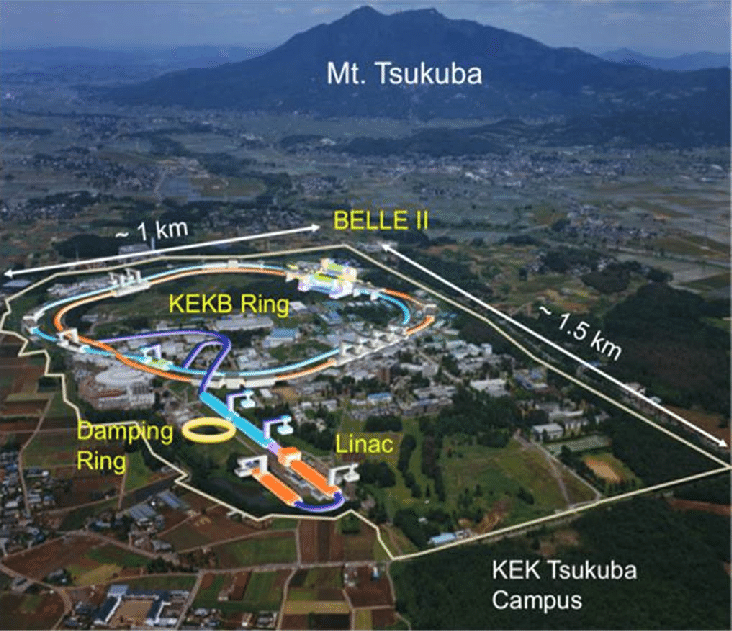
\includegraphics[width=1\textwidth]{figures/Layout-of-SuperKEKB-at-the-KEK-Tsukuba-campus.png}
      \end{columns}
   \end{frame}

   \begin{frame}{Belle~II detector}
      
\includegraphics[width=1\textwidth]{../phd_thesis/figures/experimental_setup/belle2.png}
   \end{frame}


   \begin{frame}{Data samples in B factories}
      \scriptsize\centering
      \textbf{$\sqrt{s} = 10.58~\gev$}
      
      $\epem\ra X$

      \includegraphics[width=1\textwidth]{../phd_thesis/figures/experimental_setup/corss_sections.pdf}
      \begin{itemize}
         \item \epem collissions create not only \FourS!
         \item[] $\sigma({\epem(\gamma)}) \approx 300~\nb$
         \item[] $\sigma({\FourS}) \approx 1.11~\nb$
         \item Many processes are highly different and easy to distinguish
         \item Background from $\epem\ra\qqbar$ and $\epem\ra\tautau$ often important
         \item[\ra] \textbf{all this part of Belle~II simulation}
      \end{itemize}
   \end{frame}

   %----------------------------------------------------------------------------------------
   %	B to Xs gamma
   %----------------------------------------------------------------------------------------
   \section{Belle II analysis}

   \begin{frame}{Analysis recipe}
      \scriptsize\centering
      \begin{itemize}
         \item Return to \BtoXsgamma analysis
      \end{itemize}
      
      `$\mathrm{tag~B}$' + `$\mathrm{signal~B}$' $\ra \FourS$
     
      \begin{itemize}
         \item Reconstruct all events where \textbf{one of the $B$ mesons decays hadronically}
         \item[\to] Full event intepretation algorithm used (next slide)
         \item Require a \textbf{high-energy photon from the other $B$ meson}
         \item[\to] cannot make any more requirements while maintaining an inclusive sample 
         \item[] (i.e. no $M_X$ selection)
      \end{itemize}
\textbf{Final goal:}
      \begin{equation}\nonumber
         \left.\frac{d\mathcal{B}(\BtoXsgamma)}{d\EB}\right|_i = \mathcal{U}_i \cdot \frac{N_i(\BtoXsgamma)}{\varepsilon_i N_{B}},
      \end{equation}
   \end{frame}


   \begin{frame}{Full Event Interpretation}
      \scriptsize\centering
   \begin{columns}
      \column{0.5\textwidth}
         \includegraphics[width=1\textwidth]{../phd_thesis/figures/event_reconstruction/FEI_tagging.png}
      \column{0.5\textwidth}
         \begin{itemize}
            \item Reconstructs $B$ mesons in thousands of subdecay chains
            \item Hadronic and semileptonic mode
            \item \textbf{Step 1:} Combine detector-level objects to final state particles
            \item \textbf{Step 2:} Combine final state particles to intermediate particles
            \item \textbf{Step 3:} Combine final/intermediate state particles to other intermediate particles or $B$ mesons
            \item \textbf{Step 4:} Repeat step 3 for all decay chains.
         \end{itemize}
      
   \end{columns}
\begin{itemize}
   \item Trained on simulated data but calibrated on data samples!
   \item[\ra]\textbf{end up with $B^+$ and $B^0$ candidates and a probability score \feiProb for each}
\end{itemize}   

\vspace{10pt}

Tag quality variables:
\vspace{-5pt}
\begin{equation*}
   \underbrace{\Mbc = \sqrt{(\sqrt{s}/2)^2 - (p^*_B)^2}}_{\text{beam-constrained mass}}; \quad\quad \Delta E = \sqrt{s}/2 - E_{B}^*;
\end{equation*}


\end{frame}

\begin{frame}{Reconstructed samples}
   \scriptsize
   \begin{itemize}
      \item Because of tagging, $B$ meson rest frame attainable
      \item[\ra] energy provided in the signal $B$ meson rest frame
      \item $\EB>1.4~\gev$ threshold adopted
      \item[\ra] compromise between background and signal ratio
   \end{itemize}
   \begin{columns}
      \column{0.5\textwidth}
      \includegraphics[width=1\textwidth]{../phd_thesis/figures/event_reconstruction/Bp_tagged_background.pdf}
      \column{0.5\textwidth}
      \includegraphics[width=1\textwidth]{../phd_thesis/figures/event_reconstruction/Bz_tagged_background.pdf}
   \end{columns}
   \begin{itemize}
      \item[\ra] \textbf{non-}$\bm{\Upsilon(4S)}$ \textbf{processes dominant!}
   \end{itemize}
\end{frame}

\begin{frame}{Main photon background sources}
\centering\scriptsize
      \includegraphics[width=0.5\textwidth]{../phd_thesis/figures/event_selection/Bp_photon_sources.pdf}

      \begin{itemize}
         \item Shown only for $B^+$ here, but similar for $B^0$
         \item Remaining sources correspond to 0.5\%-3\% each 
      \end{itemize}

      \begin{tikzpicture}[remember picture, overlay]
         \node[] (show) at (5,5) {};
         \node[] (showend) at (2,5) {};

         \draw [->,>=stealth] (show) -- (showend);

      \end{tikzpicture}

\end{frame}

\begin{frame}{\piz and $\eta$ suppression}
   \scriptsize\centering
\begin{itemize}
   \item $\piz\ra\g\g$ and $\eta\ra\g\g$ mimic the signal (high-$E$ $\gamma$ and low-$E$ $\gamma$)
   \item \textbf{Combine all lower-energy photons with the high-energy photon candidate}
   \item Use multivariate methods to evaluate the compatibility of the combination with a decay from \piz or $\eta$
\end{itemize}
\begin{columns}
   \column{0.5\textwidth}
   \includegraphics[width=1\textwidth]{../phd_thesis/figures/event_selection/Bp_piVeto.pdf}
   \column{0.5\textwidth}
   \includegraphics[width=1\textwidth]{../phd_thesis/figures/event_selection/Bz_etaVeto_nopi.pdf}
\end{columns}
\begin{itemize}
   \item[\ra] Validated in data using $B^+\to \bar{D}^0[\to K^+\pi^-]\pi^+$ and $B^0\to D^-[\to K^+\pi^-\pi^-]\pi^+$ decays
\end{itemize}
\end{frame}

\begin{frame}{Photon misidentification}
\centering   \scriptsize


\begin{itemize}
   \item Photon misidentification rate is small (96\% of photons are true photons)
   \item Some hadrons leave clusters which are misidentified
\end{itemize}

\vspace{5pt}

Multivariate tool, which parametrises the shower shape in terms of Zernike polynomial moments:

\vspace{5pt}

\includegraphics[width=0.5\textwidth]{../phd_thesis/figures/event_selection/Bp_zernikeMVA_mcPDG.pdf}

\begin{itemize}
   \item[\ra] successfully separates photons/non-photons
\end{itemize}

\end{frame}

\begin{frame}{Suppressing \qqbar events}
   \centering\scriptsize
   \begin{itemize}
      \item Up to now we only talked photon backgrounds
      \item As seen at the beginning \textbf{many candidates originate in} {\boldmath$\epem\ra\qqbar$} \textbf{processes}
      \item[\ra] Continuum process suppression can be used to clean up false \g candidates
   \end{itemize}

   \includegraphics[width=0.5\textwidth]{../phd_thesis/figures/continuum_suppression/figure_continuum_suppression_event_shapes.pdf}

\begin{itemize}
\item $B$ factory experiments developed many ways to \textbf{parametrise the decay topology differences}
\item They can be combined using a \textbf{boosted decision tree}
\item \textbf{Problem:} decay topology is defined by particles in it 
\item[\ra] that \textbf{includes the $X_s$ system!}
\end{itemize}

\end{frame}

\begin{frame}{Continuum suppression features}

   \scriptsize\centering

   \begin{itemize}
      \item More than 70 features are tested
      \item[\ra] here an example is shown
   \end{itemize}

   \begin{itemize}
      \item \textbf{Test 1}: test if the feature is biasing to the \EB, \Estar, \Mbc  
      \item[\ra] evaluate Jensen-Shannon distance in slices of the feature
   \end{itemize}

   \includegraphics[width=0.8\textwidth]{../phd_thesis/figures/appendices/continuum_suppression_features/thrust/Btag_cosTBTO_bias_tested.pdf}


   \begin{itemize}
      \item \textbf{Test 2}: test if the feature is described correctly in Data
      \item[\ra] use data with $\sqrt{s}-60~\mev$ (no \FourS events)
   \end{itemize}



   \includegraphics[width=0.3\textwidth]{../phd_thesis/figures/appendices/continuum_suppression_features/datamc_agreement_tests/Btag_cosTBTO_agreement_tested.pdf}

\end{frame}

\begin{frame}{Continuum suppression training}
   \scriptsize\centering
   Converge to 26 training features, and evaluate the boosted decision tree training:

   \begin{columns}
      \column{0.5\textwidth}
      \includegraphics[width=0.9\textwidth]{../phd_thesis/figures/continuum_suppression/roc_curve.png}
      \includegraphics[width=0.9\textwidth]{../phd_thesis/figures/continuum_suppression/separation_curves.pdf}


      \column{0.5\textwidth}
      \includegraphics[width=0.9\textwidth]{../phd_thesis/figures/continuum_suppression/feature_importance.pdf}

   \end{columns}
\end{frame}

\begin{frame}{Selection optimisation}
\centering\scriptsize

\begin{itemize}
   \item The previously presented selections are optimised using a Punzi figure-of-merit
\end{itemize}

\begin{equation}\nonumber
   \mathrm{FOM}_{\mathrm{Punzi}}= \frac{\mathsf{S}}{\mathsf{S}_0} \frac{1}{\frac{3}{2}+\sqrt{\mathsf{B}}}.
\end{equation}

\begin{tabular}{|l|c|}
      \hline
      Variable  & Threshold chosen \\
      \hline
      \ZMVA                      & $>0.6$\\
      \piVeto                    & $<0.4$\\
      \etaVeto                   & $<0.4$\\
      $\mathtt{BDT~output}$      & $>0.8$\\
      \hline
\end{tabular}

\vspace{5pt}

\begin{columns}
   \column{0.5\textwidth}
   \centering
   \includegraphics[width=0.85\textwidth]{../phd_thesis/figures/final_optimisation/Bp_tagged_background_optimal.pdf}
   \column{0.5\textwidth}
   \centering
   \includegraphics[width=0.85\textwidth]{../phd_thesis/figures/final_optimisation/Bz_tagged_background_optimal.pdf}
\end{columns}


\end{frame}

\begin{frame}{Best tag-side candidate selection}
\scriptsize\centering
   \begin{itemize}
      \item    FEI produces up to 20 candidates in each event!
      \item[\ra] Choose the best tag-side candidate based on \feiProb
   \end{itemize}

\begin{columns}
   \column{0.5\textwidth}
   \centering
   \includegraphics[width=0.85\textwidth]{../phd_thesis/figures/best_tag_selection/bp_Mbc_with_random_best_tag_selection.pdf}
   \column{0.5\textwidth}
   \centering
   \begin{tikzpicture}[remember picture, overlay]
      \node[] (img) {\includegraphics[width=0.85\textwidth]{../phd_thesis/figures/best_tag_selection/bp_continuum_Mbc_with_random_best_tag_selection.pdf}
      };
      \node[] at (-0.5,-0.2) (img2)  {\scriptsize$\epem\ra\qqbar$ only};
   \end{tikzpicture}

\end{columns}

\begin{itemize}
   \item Motivates to choose the highest \feiProb candidate
   \item What about the cases where there is \feiBp and \feiBz candidates in the same event?
   \item[\ra] in such cases, the correctly charged candidate has a much higher \feiProb
\end{itemize}

\end{frame}

\begin{frame}{Good tag-B mesons}
   \centering\scriptsize
   \begin{itemize}
      \item The goal is not to reconstruct the tag side:
      \item Only to infer the charge, momentum and flavour of the signal side.
      \item How to define the criterion for that?
      \item[\ra] Compare \Mbc distributions of different reconstruction errors
   \end{itemize}

   \begin{columns}
      \column{0.5\textwidth}
      \centering
      \includegraphics[width=0.85\textwidth]{../phd_thesis/figures/best_tag_selection/goodbad_tag_comparison.pdf}
      \column{0.5\textwidth}
      \centering
      \includegraphics[width=0.85\textwidth]{../phd_thesis/figures/best_tag_selection/isSig_tag_comparison.pdf}
   \end{columns}


\end{frame}

\begin{frame}{Fitting the tag-side \Mbc distribution}
\scriptsize\centering

\begin{itemize}
   \item Based on previous finding, all collected data can be split in the following categories:
\end{itemize}

\resizebox{0.7\textwidth}{!}{    
   \begin{tabular}{lc}
   \toprule
       Component & Model in fit \\
       \midrule
        {\color{ForestGreen} \epem\ra\BB well-reconstructed} & Crystal Ball  \\
        {\color{Bittersweet} \epem\ra\BB combinatorial} & Chebyshev polynomial, 5th order\\
        {\color{Bittersweet} \epem\ra\qqbar events} & Argus function\\
   \end{tabular}
   }

   \vspace{10pt}

\begin{itemize}
   \item Example fits on the full dataset ($\EB>1.4~\gev$)
\end{itemize}

   \begin{columns}
      \centering
      \column{0.33\textwidth}
      \includegraphics[width=1\textwidth]{../phd_thesis/figures/fitting/mbc_good_tags_fit.pdf}

      \column{0.33\textwidth}
      \includegraphics[width=1\textwidth]{../phd_thesis/figures/fitting/mbc_combinatorial_tags_fit.pdf}

      \column{0.33\textwidth}
      \includegraphics[width=1\textwidth]{../phd_thesis/figures/fitting/mbc_continuum_tags_fit.pdf}

   \end{columns}

   \begin{itemize}
      \item [\ra] Use these PDFs to build a fitting model
   \end{itemize}

    \begin{tikzpicture}[remember picture, overlay]
      \node[fill, white] (init) at (-5,5) {\color{black} discard};
      \node[] (inittwo) at (-4.6,4.9) {};
      \node[] (init2) at (-5,5.5) {accept};
      
      \node[] (end1) at (-4,5.2) {};
      \node[] (end2) at (-4,5.5) {};
      \node[] (end3) at (-4,4.8) {};
      
      \draw[-stealth] (init) -- (end1);
      \draw[-stealth] (inittwo) -- (end3);
      \draw[-stealth] (init2) -- (end2);
      \end{tikzpicture}
\end{frame}

\begin{frame}{Fit binning}
\small\scriptsize

Optimise based on statistical significance figure of merit studies:

\begin{itemize}
   \item 11 fitting intervals to extract \EB spectrum:\\
   \ra $1.4-1.8~\gev$ : two 200~\mev wide (control-region for fit)\\
   \ra $1.8-2.7~\gev$ : one 200~\mev and seven 100~\mev wide \textbf{(signal region)} \\
   \ra $2.7~\gev+$  \hspace{14.5pt}: one `overflow' bin (control region for fit)\\
   \item The \textbf{fit is performed using the three PDFs} in every interval
\end{itemize}

Fits on 1.6~\invab of simulation (four examples):

\begin{columns}
   \column{0.5\textwidth}
   \centering
   \includegraphics[width=0.7\textwidth]{../phd_thesis/figures/fitting/fits/full_MbcFit_1p6to1p8ppdf.pdf}
   \includegraphics[width=0.7\textwidth]{../phd_thesis/figures/fitting/fits/full_MbcFit_2p0to2p1ppdf.pdf}

   \column{0.5\textwidth}
   \centering
   \includegraphics[width=0.7\textwidth]{../phd_thesis/figures/fitting/fits/full_MbcFit_2p3to2p4ppdf.pdf}
   \includegraphics[width=0.7\textwidth]{../phd_thesis/figures/fitting/fits/full_MbcFit_2p5to2p6ppdf.pdf}


\end{columns}

\begin{tikzpicture}[remember picture, overlay]
   \node[] at (6,3) (img) {\includegraphics[width=0.2\textwidth]{../phd_thesis/figures/fitting/legend.png}};
\end{tikzpicture}




\end{frame}

\begin{frame}{Fit validity on smaller data sets}
   \scriptsize\centering
   \begin{itemize}
      \item Fit prepared on 1.6~\invab
      \item But Belle~II data is only 189~\invfb
      \item[\ra] test stability on smaller data sample (1/10th)
   \end{itemize}

      \includegraphics[width=0.9\textwidth]{../phd_thesis/figures/mc_validation/extracted_signal_generic_mc.pdf}
  \begin{itemize}
   \item[\ra] irrespective of background levels, consistent fit result
  \end{itemize}
\end{frame}

\begin{frame}{Remaining background}
\scriptsize\centering
   \begin{itemize}
      \item At this stage:
      \item[\ra] But still the result does not look like a photon energy spectrum!   
      \item[\ra] remaining background removed in a simulation reliant way
      \item[\ra] repeat the fit on simulation, but with \BtoXsgamma events removed
      \item[\ra] Subtract peaking component!  
   \end{itemize}


   \includegraphics[width=0.9\textwidth]{../phd_thesis/figures/mc_validation/subtracted_signal_generic_mc.pdf}

   \begin{itemize}
      \item Linearity tests and correlation studies also performed
      \item[\ra] all results points to the fact that the fitter is an unbiased estimator
   \end{itemize}

\end{frame}




\begin{frame}{Simulation-to-data calibration}

   \scriptsize\centering
   
   \begin{itemize}
      \item Reliance on many different tools and background modelling
      \item Need to ensure adequate agreement between data and simulation
   \end{itemize}

   \vspace{10pt}

  Main supplementary calibration and modelling studies performed:

   \begin{itemize}
      \item FEI \hspace{81pt} $\Rightarrow$ $B\to X_c \ell \nu$ 
      \item \piz and $\eta$ veto tool \hspace{27pt}  $\Rightarrow$ $B^+\to \bar{D}^0\pi^+$ and $B^0\to D^-\pi^+$
      \smash{\raisebox{.5\dimexpr1\baselineskip+2\itemsep+1\parskip}{$\left.\rule{0pt}{.5\dimexpr2\baselineskip+3\itemsep+3\parskip}\right\}\textbf{Other Belle~II analyses}$}}
      \item Photon detection efficiency  $\Rightarrow$ $\epem\ra\mumu(\gamma)$ \hspace{27pt} \textbf{\}Separate analysis performed}
      \item Post-fit background \hspace{24pt} $\Rightarrow$ world average $\mathcal{B}$ variations \hspace{15pt} \textbf{\}Study for this analysis}
   \end{itemize}

   \vspace{10pt}

   \ra FEI calibration brings $\sim 5\%$ error\\
   \ra \piz and $\eta$ veto tool add a $\sim 5-10\%$ uncertainty\\
   \ra Other calibration uncertainties $\mathcal{O}(1\%)$\\

\end{frame}

\begin{frame}{Data-to-simulation validation: off-resonance sample}
\scriptsize\centering
   \begin{itemize}
      \item Once appropriate corrections are calculated: validate the simulation using data
      \item Using a sample collected 60~\mev below the \FourS
      \item[\ra] $\epem\ra\qqbar$ validation
   \end{itemize}
\centering
        \includegraphics[width=0.55\textwidth]{../phd_thesis/figures/data_validation/Bboth_offresonance_EB.pdf}

        \begin{itemize}
         \item[\ra] excellent \EB agreement
         \item[\ra] however, off-resonance \Mbc is not comparable to on-resonance \Mbc
        \end{itemize}

\end{frame}

\begin{frame}{Data-to-simulation validation: inverted continuum}
   \scriptsize\centering
   \begin{itemize}
      \item Once appropriate corrections are calculated: validate the simulation using data
      \item Flip \texttt{BDT output} of continuum suppression
      \item[\ra]  $\epem\ra\qqbar$ validation with valid \Mbc
   \end{itemize}

   \begin{columns}
      \column{0.5\textwidth}
      \centering
         \includegraphics[width=0.85\textwidth]{../phd_thesis/figures/data_validation/Bboth_qqbar_enhanced_eb.pdf}

      \column{0.5\textwidth}
      \centering
         \includegraphics[width=0.85\textwidth]{../phd_thesis/figures/data_validation/Bboth_qqbar_enhanced_mbc.pdf}

   \end{columns}

   \begin{itemize}
      \item Excellent agreement of \EB
      \item Problematic for \Mbc!
   \item[\ra] related to the fact that $\sqrt{s}$ may vary during data taking
      \item[\ra] cannot be captured by data taking period independent simulation
   \end{itemize}

\end{frame}

\begin{frame}{Data-to-simulation validation: inverted continuum}
   \scriptsize\centering
   \begin{itemize}
      \item Once appropriate corrections are calculated: validate the simulation using data
      \item Flip \texttt{BDT output} of continuum suppression
      \item[\ra]  $\epem\ra\qqbar$ validation with valid \Mbc
   \end{itemize}

   \begin{columns}
      \column{0.5\textwidth}
      \centering
         \includegraphics[width=0.85\textwidth]{../phd_thesis/figures/data_validation/Bboth_qqbar_enhanced_eb.pdf}
      \column{0.5\textwidth}
      \centering
         \includegraphics[width=0.85\textwidth]{../phd_thesis/figures/data_validation/Bboth_qqbar_enhanced_mbccorrected.pdf}
   \end{columns}

   \begin{itemize}
      \item Excellent agreement of \EB
      \item Problematic for \Mbc!
      \item[\ra] need to modify the \Mbc in simulation:  
   \end{itemize}
   \begin{equation*}
      \sqrt{s}^{\mathrm{MC}} \xrightarrow[\mathrm{in~50\%~of~cases}]{\mathrm{replace~with~weighted~probability}} \sqrt{s}^{\mathrm{DATA}}
   \end{equation*}

   \begin{itemize}
   \item[\ra] e.g. if x value is set for 30\% of data, then the weighted probability for x is 0.3
\end{itemize}
\end{frame}

\begin{frame}{Data-to-simulation validation: inverted \piz and $\eta$}
   \scriptsize\centering
   \begin{itemize}
      \item Once appropriate corrections are calculated: validate the simulation using data
      \item Flip \piVeto and \etaVeto
      \item[\ra]  $\BB$ background validation ($B\to X \piz$ and $B\to X \eta$)
   \end{itemize}

   \begin{columns}
      \column{0.5\textwidth}
      \includegraphics[width=0.85\textwidth]{../phd_thesis/figures/data_validation/Bboth_bbbar_enhanced_eb.pdf}
      \column{0.5\textwidth}
      \includegraphics[width=0.85\textwidth]{../phd_thesis/figures/data_validation/Bboth_bbbar_enhanced_mbccorrected.pdf}
   \end{columns}

   \begin{itemize}
      \item Now only the `corrected' \Mbc is used!
      \item Assign \textbf{the difference with, without corrected \Mbc as fit model uncertainty}!
   \end{itemize}

\end{frame}

\begin{frame}{Data-to-simulation validation: sidebands}
   \scriptsize\centering
   \begin{itemize}
      \item Once appropriate corrections are calculated: validate the simulation using data
      \item The sideband region (\EB<1.8~\gev and \EB>2.7~\gev) with full signal selection
   \end{itemize}

   \begin{columns}
      \column{0.5\textwidth}
      \includegraphics[width=0.85\textwidth]{../phd_thesis/figures/data_validation/Bboth_sidebands_eb.pdf}
      \column{0.5\textwidth}
      \includegraphics[width=0.85\textwidth]{../phd_thesis/figures/data_validation/sidebands_mbc_1.pdf}
   \end{columns}

   \begin{itemize}
      \item Now only the `corrected' \Mbc is used!
      \item Not only \Mbc discrepancy but also endpoint discrepancy
   \end{itemize}

\end{frame}

\begin{frame}{Data-to-simulation validation: sidebands}
   \scriptsize\centering
   \begin{itemize}
      \item Once appropriate corrections are calculated: validate the simulation using data
      \item The sideband region (\EB<1.8~\gev and \EB>2.7~\gev) with full signal selection
   \end{itemize}

   \begin{columns}
      \column{0.5\textwidth}
      \includegraphics[width=0.85\textwidth]{../phd_thesis/figures/data_validation/Bboth_sidebands_zmva.pdf}
      \column{0.5\textwidth}
      \includegraphics[width=0.85\textwidth]{../phd_thesis/figures/data_validation/sidebands_mbc_nozmva_1.pdf}
   \end{columns}

   \begin{itemize}
      \item \text{zernikeMVA} discrepancy?
      \item[\ra] improved agreement when no \texttt{zernikeMVA} is used
      \item[\ra] more studies are needed to pinpoint the exact cause of this discrepancy
      \item[\ra] seems to be a this-analysis-specific background
   \end{itemize}

\end{frame}

\begin{frame}{Data-to-simulation validation: sidebands}
   \scriptsize\centering
   \begin{itemize}
      \item Once appropriate corrections are calculated: validate the simulation using data
      \item The sideband region (\EB<1.8~\gev and \EB>2.7~\gev) with full signal selection
   \end{itemize}

   \begin{columns}
      \column{0.33\textwidth}
      \centering
      \includegraphics[width=0.85\textwidth]{../phd_thesis/figures/data_validation/sidebands_fit/DATA_MbcFit_1p4to1p6ppdf.pdf}
      \column{0.33\textwidth}
      \centering
      \includegraphics[width=0.85\textwidth]{../phd_thesis/figures/data_validation/sidebands_fit/DATA_MbcFit_1p6to1p8ppdf.pdf}
      \column{0.33\textwidth}
      \centering
      \includegraphics[width=0.85\textwidth]{../phd_thesis/figures/data_validation/sidebands_fit/DATA_MbcFit_2p7to5p0ppdf.pdf}
   \end{columns}

   \begin{itemize}
      \item $\mathcal{N}_{\mathrm{DATA}}/\mathcal{N}_{\mathrm{MC}}\approx 1.087\pm 0.080$
   \end{itemize}

   \includegraphics[width=0.45\textwidth]{../phd_thesis/figures/data_validation/sidebands_background_vs_data.pdf}

\end{frame}
\begin{frame}{Data-to-simulation validation: sidebands}
   \scriptsize\centering
   \begin{itemize}
      \item Once appropriate corrections are calculated: validate the simulation using data
      \item The sideband region (\EB<1.8~\gev and \EB>2.7~\gev) with full signal selection
   \end{itemize}

   \begin{columns}
      \column{0.5\textwidth}
      \centering
      \includegraphics[width=0.85\textwidth]{../phd_thesis/figures/data_validation/sideband_event_counts.pdf}
    \column{0.5\textwidth}
    \centering
     \includegraphics[width=0.85\textwidth]{../phd_thesis/figures/data_validation/sideband_event_counts_corrected.pdf}
   \end{columns}

   $\xrightarrow{\text{Apply an 8.7\% correction, because we expect the results here to be consistent with 0}}$

   \begin{itemize}
      \item Assign \textbf{the full correction as a systematic uncertainty}
   \end{itemize}

\end{frame}

\begin{frame}{\BtoXsgamma efficiency validation}
\scriptsize\centering
\begin{itemize}
   \item Efficiency is assumed to factorise:
\end{itemize}
\begin{equation*}
   \varepsilon_{\BtoXsgamma} = \varepsilon_{\mathrm{FEI}} \cdot \varepsilon_{\mathrm{selection}},
\end{equation*}

\vspace{-5pt}

\begin{itemize}
   \item $\varepsilon_{\mathrm{FEI}}$ calculated based on simulation + corrected using calibration factors
\end{itemize}
\begin{equation*}
   \varepsilon_{\mathrm{FEI}} = 0.00444\pm0.00015
\end{equation*}
\begin{itemize}
   \item $\varepsilon_{\mathrm{selection}}$ are calculated based on simulation + corrected:
   \begin{itemize}
      \scriptsize
      \item \piVeto and \etaVeto correction, photon detection efficiency 
      \item[\ra] calculated in separate analyses\\
      \vspace{5pt}
      \item \texttt{BDToutput}, \texttt{ZernikeMVA} by varying their selection 
      \item[\ra] variations directly in data (blinded) evaluated and assigned as uncertainty
   \end{itemize}
\end{itemize}
\includegraphics[width=0.45\textwidth]{../phd_thesis/figures/signal_validation/corrected_selection_efficiency.pdf}



\end{frame}

\begin{frame}{Unfolding}
\centering\scriptsize

\begin{itemize}
   \item Simplest approach: bin-by-bin correction
   \item[\ra] although cross-bin migrations are not taken into account
   \item[\ra] however given the statistical uncertainty this is sufficient
\end{itemize}
\begin{equation*}\label{eq:bin_by_bin_unfolding}
   x_i = y_i \cdot \frac{N_i^{\mathrm{gen}}}{N_i^{\mathrm{meas}}},
  \end{equation*}

  \begin{equation*}\label{eq:bin_by_bin_unfolding_error}
      \Delta x_i = \Delta y_i \cdot \frac{N_i^{\mathrm{gen}}}{N_i^{\mathrm{meas}}},
  \end{equation*}
\begin{itemize}
   \item Unfolding model chosen by merging the inclusive \BtoXsgamma model with $B\to\Kstar(892)\gamma$ resonance
\end{itemize}

\begin{columns}
   \centering
   \column{0.5\textwidth}
   \textbf{Model:}
   \includegraphics[width=0.85\textwidth]{../phd_thesis/figures/data_samples/hybrid_model_uncertainties.pdf}

   \column{0.5\textwidth}
   \centering
   \textbf{Unfolding} (simulation):
   \includegraphics[width=0.85\textwidth]{../phd_thesis/figures/signal_validation/reco_vs_true_spectrum.pdf}

\end{columns}


\end{frame}

% \begin{frame}{Systematic uncertainties}
%    \scriptsize\centering
%    \begin{itemize}
%       \item Summary of systematic uncertainties that are evaluates:
%       \item[\ra] Background modelling/normalisation uncertainties
%       \item[\ra] Fit model uncertainties
%       \item[\ra] Efficiency uncertainties
%       \item[\ra] Unfolding and \BtoXdgamma uncertainties   
%    \end{itemize}
% \end{frame}

\begin{frame}{Fit results -- Unblinded}
\begin{columns}
   \column{0.33\textwidth}
   \centering
   \includegraphics[width=1\textwidth]{../phd_thesis/figures/final_results/data_fits/DATA_MbcFit_1p8to2p0ppdf.pdf}
   \includegraphics[width=1\textwidth]{../phd_thesis/figures/final_results/data_fits/DATA_MbcFit_2p2to2p3ppdf.pdf}

   \column{0.33\textwidth}
   \centering
   \includegraphics[width=1\textwidth]{../phd_thesis/figures/final_results/data_fits/DATA_MbcFit_2p0to2p1ppdf.pdf}
   \includegraphics[width=1\textwidth]{../phd_thesis/figures/final_results/data_fits/DATA_MbcFit_2p3to2p4ppdf.pdf}

   \column{0.33\textwidth}
   \centering
   \includegraphics[width=1\textwidth]{../phd_thesis/figures/final_results/data_fits/DATA_MbcFit_2p1to2p2ppdf.pdf}
   \includegraphics[width=1\textwidth]{../phd_thesis/figures/final_results/data_fits/DATA_MbcFit_2p4to2p5ppdf.pdf}
\end{columns}
\begin{columns}
   \column{0.5\textwidth}
   \centering
   \includegraphics[width=0.66\textwidth]{../phd_thesis/figures/final_results/data_fits/DATA_MbcFit_2p5to2p6ppdf.pdf}
   \column{0.5\textwidth}
   \centering
   \includegraphics[width=0.66\textwidth]{../phd_thesis/figures/final_results/data_fits/DATA_MbcFit_2p6to2p7ppdf.pdf}

\end{columns}
\end{frame}

\begin{frame}{Background subtracted results}
   \centering\scriptsize
\textbf{Fit results summarised:}
\begin{columns}
   \column{0.5\textwidth}
   \centering
   \includegraphics[width=0.85\textwidth]{../phd_thesis/figures/final_results/background_vs_data_final.pdf}
   \column{0.5\textwidth}
   \centering
   \includegraphics[width=0.85\textwidth]{../phd_thesis/figures/final_results/background_vs_data_final_log.pdf}
\end{columns}
\textbf{Background subtracted:}

\begin{columns}
   \column{0.5\textwidth}
   \centering
   \includegraphics[width=0.85\textwidth]{../phd_thesis/figures/final_results/reco_spectrum_overlayed.pdf}
   \column{0.5\textwidth}
   \centering
   \includegraphics[width=0.85\textwidth]{../phd_thesis/figures/final_results/reco_spectrum_overlayed_signal_region.pdf}
\end{columns}

\end{frame}

\begin{frame}{Total and partial branching fractions}
   \centering\scriptsize
      \includegraphics[width=0.45\textwidth]{../phd_thesis/figures/final_results/partial_bfs.pdf}

      \textbf{Or numerically:}
      \vspace{5pt}

      \resizebox{1\textwidth}{!}{
         \begin{tabular}{|c|ccc||cccc|}
         \hline
         \multirow{2}{*}[-6pt]{\EB interval [\gev]} &
         \multirow{2}{*}[-6pt]{$\frac{\Delta\mathcal{B}(\BtoXsgamma)_i}{\Delta {E^B_{\g}}_{,i}} (10^{-4})$} &
         \multirow{2}{*}[-6pt]{\makecell{Statistical\\uncertainty} ($10^{-4}$)} &
         \multirow{2}{*}[-6pt]{\makecell{Systematic\\uncertainty} ($10^{-4}$)}& 
         \multicolumn{4}{c|}{Systematic uncertainty group} \\
         \cline{5-8}
         & & & &        
         \makecell{Background \\ modelling} &
         \makecell{\Mbc fit \\ model} & 
         \makecell{\BtoXsgamma \\efficiency} & 
         \makecell{Other\\uncertainties}\\
         \hline
         $1.8-2.0$  &  0.48 & $\pm0.54$ & $\pm0.64$ & 0.49 & 0.42 & 0.03 & 0.09 \\
         $2.0-2.1$  &  0.57 & $\pm0.31$ & $\pm0.25$ & 0.17 & 0.17 & 0.06 & 0.07 \\
         $2.1-2.2$  &  0.13 & $\pm0.26$ & $\pm0.16$ & 0.11 & 0.13 & 0.01 & 0.01 \\
         $2.2-2.3$  &  0.41 & $\pm0.22$ & $\pm0.10$ & 0.04 & 0.07 & 0.05 & 0.02 \\
         $2.3-2.4$  &  0.48 & $\pm0.22$ & $\pm0.10$ & 0.02 & 0.06 & 0.06 & 0.05 \\
         $2.4-2.5$  &  0.75 & $\pm0.19$ & $\pm0.14$ & 0.02 & 0.04 & 0.09 & 0.09 \\
         $2.5-2.6$  &  0.71 & $\pm0.13$ & $\pm0.10$ & 0.00 & 0.02 & 0.09 & 0.04  \\
         \hline
         \end{tabular}
     }

\end{frame}

\begin{frame}{Interated results}

   \centering\scriptsize

   \textbf{Integrated results:}

   \resizebox{1\textwidth}{!}{
  \begin{tabular}{|c|cl|}
  \hline
      \EB lower threshold [\hspace{-1pt}$\gev$] & 
      $\mathcal{B}(B\rightarrow X_s \gamma)~[10^{-4}]$ & 
      \makecell{$\mathcal{B}(B\rightarrow X_s \gamma)~[10^{-4}]$\\(extrapolated to $1.6~\gev)$}  \\
      \hline
          $1.8$  & $3.54 \pm 0.78$ (stat.) $\pm~0.83$ (syst.) & $3.65 \pm 0.80$ (stat.) $\pm 0.86$ (syst.) $\pm 0.02$ (extrap.)\\ 
          $2.0$  & $3.06 \pm 0.56$ (stat.) $\pm~0.47$ (syst.) & $3.42 \pm 0.62$ (stat.) $\pm 0.52$ (syst.) $\pm 0.06$ (extrap.)\\
          $2.1$  & $2.49 \pm 0.46$ (stat.) $\pm~0.35$ (syst.) & $2.86 \pm 0.53$ (stat.) $\pm 0.40$ (syst.) $\pm 0.08$ (extrap.)\\
      \hline
      World average (\EB>1.6~\gev) & \multicolumn{2}{c}{$3.49\pm0.19$} \\
      \hline
  \end{tabular}

}

\vspace{10pt}

\textbf{Moments of the spectrum:}

\resizebox{1\textwidth}{!}{
    \begin{tabular}{|c|cc|}
    \hline
        \EB lower threshold [\hspace{-1pt}$\gev$] & 
        $\expval**{\EB}$ [$\gev$] & $\expval**{\EB^2}$ - $\expval**{\EB}^2$ [$\gev^2$]\\
        \hline
        1.8 & 2.284 $\pm$ 0.065 (stat.) $\pm$ 0.071 (syst.)    & 0.0502 $\pm$ 0.0157 (stat.) $\pm$ 0.0176 (syst.)\\
        2.0 & 2.343 $\pm$ 0.036 (stat.) $\pm$ 0.026 (syst.)    & 0.0315 $\pm$ 0.0063 (stat.) $\pm$ 0.0045 (syst.)\\
        2.1 & 2.410 $\pm$ 0.032 (stat.) $\pm$ 0.019 (syst.)    & 0.0147 $\pm$ 0.0057 (stat.) $\pm$ 0.0036 (syst.)\\
        
        \hline
       World average: & $2.314 \pm 0.011$ & $0.0303 \pm 0.0025$ \\
       \hline

    \end{tabular}

}

\end{frame}

\begin{frame}{Comparison with existing results}
\centering\scriptsize

Extrapolation to $\EB>1.6~\gev$ 

      \includegraphics[width=0.7\textwidth]{../phd_thesis/figures/results_discussion/all_measurements_compared.pdf}

      \begin{itemize}
         \item Extrapolated results more precise but always model dependant
         \item Different experiments and theory choose different thresholds
         \item[\ra] extrapolations to a common threshold are necessary
      \end{itemize}
      
\end{frame}

\begin{frame}{Input to the theoretical calculations}
\centering\scriptsize
\begin{columns}
   \centering
   \column{0.5\textwidth}
   \centering\scriptsize

   \includegraphics[width=0.45\textwidth]{figures/babar_hadtag_spec_default_la055_a3.pdf}
   \includegraphics[width=0.45\textwidth]{figures/babar_incl_spec_default_la055_a3.pdf}
   \includegraphics[width=0.45\textwidth]{figures/babar_sem_spec_default_la055_a3.pdf}
   \includegraphics[width=0.45\textwidth]{figures/belle_spec_default_la055_a3.pdf}
   
   {\Large +}
   
   \includegraphics[width=0.85\textwidth]{../phd_thesis/figures/results_discussion/simba_partial_bfs_expectation.pdf}

   \column{0.5\textwidth}
   \centering
   \begin{itemize}
      \item Global fit of all experimental information by simba
      \item Extract shape function and its parameters
   \end{itemize}
   \includegraphics[width=0.85\textwidth]{../phd_thesis/figures/results_discussion/C7incl_mb_la055_henrikas.pdf}

\end{columns}

\begin{tikzpicture}[remember picture, overlay]
   \node (dog) at (-0.15,4.) {\LARGE $\bm{\Longrightarrow}$};
\end{tikzpicture}

\end{frame}   

\begin{frame}{Future prospects}
\scriptsize\centering
   \begin{itemize}
      \item The future holds good things!
      \item Other results already limited systematically
      \item[\ra] hadronic tag will only be limited systematically at 5-10~\invab
   \end{itemize}

\resizebox{1\textwidth}{!}{
      \begin{tabular}{|c|cccc|c|}
          \hline
          \multirow{2}{*}{Lower \EB threshold} & \multicolumn{4}{c|}{Statistical uncertainty} & \multirow{2}{*}{\makecell{Baseline (improved)\\ systematic uncertainty}} \\
          & 1~\invab& 5~\invab & 10~\invab & 50~\invab & \\
          \hline
          1.4~\gev & 10.7\% & 6.4\% & 4.7\% & 2.2\% & 10.3 \% (5.2\%)\\
          1.6~\gev & 9.9 \% & 6.1\% & 4.5\% & 2.1\% & 8.5 \% (4.2\%)\\ 
          1.8~\gev & 9.3 \% & 5.7\% & 4.2\% & 2.0\% & 6.5 \% (3.2\%)\\ 
          2.0~\gev & 8.3 \% & 5.1\% & 3.8\% & 1.7\% & 3.7 \% (1.8\%)\\ 
          \hline
      \end{tabular}
}
\end{frame}

\appendix

%----------------------------------------------------------------------------------------
%	B to Xs gamma
%----------------------------------------------------------------------------------------
\section{Appendix}

\begin{frame}

   \centering\Large

   Appendix

\end{frame}

\begin{frame}{Description of the inclusive decays}
   \scriptsize

   \begin{itemize}
      \item Fully inclusive decay rate is related to the \textbf{the parton decay rate}
      \item The $b\to s$ electroweak loop is \textbf{dominated by the top quark} 
      \item It \textbf{involves both weak and strong interactions}
      \item[\ra] energy scale $\ll\order(m_W)$
      \item[\ra] approximate weak interactions with effective point-like vertices.
   \end{itemize}

   \textbf{Effective Lagrangian:}
   \begin{equation}\nonumber
      \mathcal{L}_{\mathrm{eff}} = \frac{4G_F}{\sqrt{2}}V_{tq}^*V_{tb}\left[\sum^{8}_{i=1}\mathcal{C}_i(\mu)\mathcal{O}_i(\mu)
                                                  + \frac{V^*_{uq}V_{ub}}{V^*_{tq}V_{tb}}\sum^{2}_{i=1}\mathcal{C}_i(\mu)(\mathcal{O}_i(\mu)-\mathcal{O}_i^u(\mu))\right]
  \end{equation}

  \vspace{10pt}

  $\mathcal{C}_i$: Wilson coefficients (encode \Wpm and $Z$ interactions)
  
  $\mathcal{O}_i$: Four-quark and dipole-type operators (quark interactions)

\end{frame}

\begin{frame}{Description of the inclusive decays}
   \scriptsize

   \begin{equation}\nonumber
      \mathcal{L}_{\mathrm{eff}} = \frac{4G_F}{\sqrt{2}}V_{tq}^*V_{tb}\left[\sum^{8}_{i=1}\mathcal{C}_i(\mu)\mathcal{O}_i(\mu)
                                                  + {\underbrace{\frac{V^*_{uq}V_{ub}}{V^*_{tq}V_{tb}}}_{\substack{\approx 0.02,~\mathbf{q = s}\\\approx 0.47,~\mathbf{q = d}}}}\sum^{2}_{i=1}\mathcal{C}_i(\mu)(\mathcal{O}_i(\mu)-\mathcal{O}_i^u(\mu))\right]
   \end{equation}

\begin{itemize}
   \item For \btosgamma the second term is much less important
   \item It is relevant for higher order corrections, and for \btodgamma
\end{itemize}

\end{frame}


\begin{frame}{\safeBtoXsgamma total decay rate calculations}
\scriptsize
   \begin{itemize}
      \item That was for the \textit{parton} decay rate;
      \item[\ra] can be calculated perturbatively 
      \item Switch from partons to hadrons assuming quark-hadron duality:
   \end{itemize}

   \vspace{10pt}

   \begin{equation}\nonumber
      \Gamma(B\ra\X_s\g) = \Gamma(b\ra s\g) + \underbrace{\Delta\Gamma_{\mathrm{non-p.}}}_{\substack{\text{additional}\\\text{non-perturbative}\\\text{term}}}
  \end{equation}
  \begin{itemize}
   \item[\ra] related to the fact that the $b$ quark is non-stationary and within a $B$ meson
   \item Many such effects decrease or `average out' over the totality of the spectrum
   \item However, others remain: e.g. around $\Egamma<1.5~\gev$ non-perturbative \ccbar contributions become relevant 
     \end{itemize}

     \textbf{A convention $\Egamma>1.6~\gev$ chosen in inclusive decay rate calculations}

\end{frame}

\begin{frame}{\safeBtoXsdgamma spectrum calculations}
\scriptsize
   Non-perturbative effects more complicated if the partial decay rates are considered

   \begin{columns}
      \column{0.5\textwidth}
      \includegraphics[width=1\textwidth]{../phd_thesis/figures/theory/xsgamma_theory_to_experiment.png}
      \column{0.5\textwidth}
      \includegraphics[width=1\textwidth]{../phd_thesis/figures/theory/xsgamma_theory_components.png}
   \end{columns}

   \begin{itemize}
      \item Use soft-collinear effective field theory:
   \end{itemize}
   \begin{equation}\nonumber
      d\Gamma \propto \mathcal{H} \times \mathcal{J} \otimes \mathcal{S}.
  \end{equation}
  which splits the calculation of:
  \begin{itemize}
   \item[] {\color{red}$\mathcal{H}$: effective hard interaction (perturbative)}
   \item[] {\color{blue}$\mathcal{J}$: collinear particle interactions (perturbative)}
   \item[] {\color{orange}$\mathcal{S}$: soft particle interactions}
  \end{itemize}

\vspace{-10pt}

\begin{flushright}
   \tiny \textbf{Credit to Frank Tackmann for the illustrations.}
\end{flushright}

\end{frame}

\begin{frame}{\safeBtoXsdgamma spectrum calculations}
   \scriptsize
      Non-perturbative effects more complicated if the partial decay rates are considered
   
      \begin{columns}
         \column{0.5\textwidth}
         \includegraphics[width=1\textwidth]{../phd_thesis/figures/theory/xsgamma_theory_to_experiment.png}
         \column{0.5\textwidth}
         \includegraphics[width=1\textwidth]{../phd_thesis/figures/theory/xsgamma_theory_components.png}
      \end{columns}
   
      \begin{itemize}
         \item Use soft-collinear effective field theory:
      \end{itemize}
      \begin{equation}\nonumber
         d\Gamma \propto \mathcal{H} \times \mathcal{J} \otimes \mathcal{S}.
     \end{equation}

     \vspace{-10pt}
     \begin{itemize}
      \item It is assumed that:
     \end{itemize}
     \begin{equation}\nonumber
      \mathcal{S} \equiv \underbrace{\mathcal{S}_p}_{\substack{\text{perturbative}\\\text{partonic soft function}}} \otimes \underbrace{\mathcal{F}}_{\substack{\text{non perturbative}\\\textbf{shape function}}}
     \end{equation}
     \begin{itemize}
      \item[\ra] the theory is capable to separate perturbative and non-perturbative terms 
     \end{itemize}

   \vspace{-5pt}
   
   \begin{flushright}
      \tiny \textbf{Credit to Frank Tackmann for the illustrations.}
   \end{flushright}
   
   \end{frame}

   \begin{frame}{\BtoXsgamma spectrum and the shape function}
      \scriptsize
      \begin{itemize}
         \item The shape function $\mathcal{F}$ encodes the Fermi motion of the $b$ and is therefore \textbf{universal for the} \bm{$B$} \textbf{meson}\footnote[1]{\tiny however, more shape function need to be introduced at higher orders}
         \item \textbf{Crucial input for other analyses}, e.g. $|V_{ub}|$ measurements with $B\to\X_u\ell\nu$, using phase space selection to separate $B\to\X_c\ell\nu$ states
      \end{itemize}

      \textbf{So how to evaluate it?}

   \end{frame}


   \begin{frame}{\BtoXsgamma spectrum and the shape function}
      \scriptsize
      \begin{itemize}
         \item The shape function $\mathcal{F}$ encodes the Fermi motion of the $b$ and is therefore \textbf{universal for the} \bm{$B$} \textbf{meson}\footnote[1]{\tiny however, more shape function need to be introduced at higher orders}
         \item \textbf{Crucial input for other analyses}, e.g. $|V_{ub}|$ measurements with $B\to\X_u\ell\nu$, using phase space selection to separate $B\to\X_c\ell\nu$ states
      \end{itemize}

      \textbf{So how to evaluate it?}
      \begin{itemize}
         \item[\ra] you have to use experimental information: 
         \item[\ra] \BtoXsgamma is a highly suitable channel for this
      \end{itemize}

   \end{frame}

   \begin{frame}{\BtoXsgamma spectrum and the shape function}
      \scriptsize
      It can be shown that the moments of photon energy spectrum relate to
      \begin{equation}\nonumber
         \expval**{\Egamma} \sim m_b/2+\order(\Lambda_{\mathrm{QCD}}); \quad \expval**{\Egamma^2}-\expval**{\Egamma}^2 \sim \lambda_1/3+\order(\Lambda_{\mathrm{QCD}}),
     \end{equation}
     with:
     \begin{itemize}
      \item [] $m_b$: $b$ quark pole MASS
      \item [] $\lambda_1$: $b$ quark kinetic energy parameter
      \item [] etc. for higher moments
     \end{itemize}
   $\mathcal{F}$ can be parametrised in terms of these quantities!
   \end{frame}


   \begin{frame}{Kagan-Neubert model}
      \scriptsize
      \textbf{Kagan-Neubert} model is often used for experimental analyses:
      \begin{equation}\nonumber
         \mathcal{F}(x) = N\left(1-\frac{x}{m_B-m_b}\right)^a\exp{(1+a)\frac{x}{m_B-m_b}},
     \end{equation}
     and the parameter $a$ is also related to the second moment of the shape function.

     Then the spectrum can be described by two parameters: $m_b$ and $\lambda_1$;

     \begin{itemize}
      \item[\ra] Measure the moments of \BtoXsgamma spectrum to obtain a better description 
     \end{itemize}

   \end{frame}

   \begin{frame}{SIMBA global fit of \BtoXsgamma}
      \scriptsize
      \textbf{SIMBA} collaboration: 
      Combine all the information available from experimental measurements
      \begin{itemize}
       \item[\ra] global fit of \BtoXsgamma measurements to determine $m_b$ and $\lambda_1$
      \end{itemize}

      \begin{columns}
         \centering
         \column{0.5\textwidth}
         \includegraphics[width=0.7\textwidth]{figures/babar_hadtag_spec_default_la055_a3.pdf}
         \includegraphics[width=0.7\textwidth]{figures/babar_incl_spec_default_la055_a3.pdf}
         \column{0.5\textwidth}
         \includegraphics[width=0.7\textwidth]{figures/babar_sem_spec_default_la055_a3.pdf}
         \includegraphics[width=0.7\textwidth]{figures/belle_spec_default_la055_a3.pdf}
      \end{columns}
      \begin{flushright}
         {\tiny\textbf{Phys.Rev.Lett. 127 (2021) 10, 102001}}
      \end{flushright}
   \end{frame}

\begin{frame}{Beyond the Standard Model}
   \scriptsize
   Only heavy particles are expected, in other words, the effective Lagrangian would be modified as:
   \begin{equation}\nonumber
      \mathcal{C}_i^{\mathrm{SM}} \ra \mathcal{C}_i^{\mathrm{SM}} + \Delta\mathcal{C}_i^{\mathrm{BSM}}.
   \end{equation}
   Some models may propose $\Delta\mathcal{C}_j^{\mathrm{BSM}}$, where $\mathcal{C}_j^{\mathrm{SM}}=0$

\vspace{10pt}
   In no particular order, some (but surely not all) theories which propose such modifications:
   \begin{itemize}
      \item two-Higgs-doublet models $\leftarrow$ \textbf{to my knowledge, the most studied}
      \item minimal supersymmetric models with minimal flavour violation
      \item and left-right symmetric models
      \item general minimal-supersymmetric theories
      \item models with extra dimensions
      \item the littlest Higgs models
      \item 331 models
   \end{itemize}
\end{frame}

\begin{frame}{\safeBtoXsgamma measurement techniques}
   \scriptsize
   \begin{columns}
      \centering
      \column{0.4\textwidth}
      \pgfdeclarelayer{bg}    % declare background layer
\pgfsetlayers{bg,main}  % set the order of the layers (main is the standard layer)
\begin{tikzpicture}[rotate=90]

    % NODES
    
    % Initial state
    \node [circle, minimum size=1.2cm, draw=white, ultra thick]    (collision) {} ;
    % \node [] (collision) {} ;
    \node [] (collisiontext) [below=0.03cm of collision.west] {\FourS};
    \node [] (eminus)     [left=2cm of collision.center] {};
    \node [] (eplus)     [right=1.5cm of collision.center] {};
    \node [] (eplusabove) [above=0.1cm of eplus] {};
    \node [] (eminusabove) [above=0.1cm of eminus] {};
    \node [] (eminustext)     [right=0.3cm of eminusabove, text=blue] {\en};
    \node [] (eplustext)     [left=0.3cm of eplusabove, text=red] {\ep};
    
    % BB bar
    \node [] (bbarup) [above=0.7cm of collision.north east] {};
    \node [] (bbardown) [below=0.5cm of collision.south east] {};
    \node [] (bbarup_text) [right=0.05cm of bbarup.center] {$\B_{\mathrm{sig}}$};
    \node [] (bbardown_text) [right=0.05cm of bbardown.center] {$\B_{\mathrm{tag}}$};
    
    % Xs gamma
    %%gamma
    \node [] (gamma_int) [left=0.5cm of bbarup.center] {};
    \node [] (gamma) [above=1cm of gamma_int.center] {};
    \node [] (gammatext) [left=0.05cm of gamma.center] {$\gamma$};
    %%xs
    \node [] (Xs_int) [right=0.5cm of bbarup.center] {};
    \node [] (Xs) [above=0.5cm of Xs_int.center] {};
    \node [] (Xstext) [left=0.05cm of Xs.center] {$X_{s}$};
    %%xs daughters
    \node [] (Xsd1_int) [left=0.05cm of Xs.center] {};
    \node [] (Xsd1) [above=0.5cm of Xsd1_int.center] {};
    \node [] (Xsd2_int) [right=0.2cm of Xs.center] {};
    \node [] (Xsd2) [above=0.4cm of Xsd2_int.center] {};
    \node [] (Xsd3_int) [right=0.35cm of Xs.center] {};
    \node [] (Xsd3) [above=0.2cm of Xsd3_int.center] {};
    
    % Tag side
    
    % first generation
    \node [] (D0_int) [left=0.35cm of bbardown.center] {};
    \node [] (D0) [below=0.65cm of D0_int.center] {};
    \node [] (pi0_int) [right=0.3cm of bbardown.center] {};
    \node [] (pi0) [below=0.6cm of pi0_int.center] {};
    
    %second generation
    \node [] (Kp_int) [left=0.25cm of D0.center] {};
    \node [] (Kp) [below=0.65cm of Kp_int.center] {};
    \node [] (pim_int) [right=0.1cm of D0.center] {};
    \node [] (pim) [below=0.6cm of pim_int.center] {};

    \node [] (g1_int) [left=0.2cm of pi0.center] {};
    \node [] (g1) [below=0.65cm of g1_int.center] {};
    \node [] (g2_int) [right=0.15cm of pi0.center] {};
    \node [] (g2) [below=0.6cm of g2_int.center] {};
    
    %\node [] (hadron text) [below=0.05cm of bbardown.center] {\scriptsize hadrons};
    
    % Colored overal blocks
    
    \node [] (sigside) [above=0.8cm of bbarup] {};
    \node [] (tagside) [below=0.8cm of bbardown] {};
    \node [] (tagside_right) [right=0.2cm of tagside] {};
    
    \node [] (sigsidetext) [above=0.1cm of sigside] {\scriptsize Signal side};
    \node [] (tagsidetext) [below=0.3cm of tagside_right, text width = 2cm] {\centering\scriptsize Tag side};
    
    \begin{pgfonlayer}{bg}    % select the background layer
    \node [rectangle, fill=green!20, text width=2cm, text centered, rounded corners, minimum height=1.7cm] (Signal_Side) at (sigside) {};
    \node [rectangle, fill=blue!20, text width=2cm, text centered, rounded corners, minimum height=1.7cm] (Signal_Side) at (tagside) {};
    \end{pgfonlayer}

    

    
    % LINES
    
    % Initial state
    \draw [-Triangle, blue, thick] (eminus) -- (collision.center);
    \draw [-Triangle, red, thick] (eplus) -- (collision.center);
    
    % BB bar
    \draw[-Triangle, thick] (collision.center) -- (bbarup.center);
    \draw[-Triangle, thick] (collision.center) -- (bbardown.center);
    
    % Xs gamma
    \draw[-Triangle, thick, purple, dashed] (bbarup.center) -- (gamma.center);
    \draw[-Triangle, thick] (bbarup.center) -- (Xs.center);
    \draw[-Triangle, thick] (Xs.center) -- (Xsd1.center);
    \draw[-Triangle, thick] (Xs.center) -- (Xsd3.center);
    \draw[-Triangle, thick] (Xs.center) -- (Xsd2.center);
    
    % Tag side
    \draw[-Triangle, thick] (bbardown.center) -- (D0.center);
    \draw[-Triangle, thick] (bbardown.center) -- (pi0.center);

    \draw[-Triangle, thick] (D0.center) -- (Kp.center);
    \draw[-Triangle, thick] (D0.center) -- (pim.center);
    \draw[-Triangle, thick, dashed] (pi0.center) -- (g1.center);
    \draw[-Triangle, thick, dashed] (pi0.center) -- (g2.center);
    

    
\end{tikzpicture}
      \column{0.6\textwidth}
      \centering
      \textbf{Sum of exclusive}
      \begin{itemize}
         \item Reconstruct specific $X_s$ states:
         \begin{itemize}
            \scriptsize
            \item $K^*(892)$
            \item $K^+p^-$\\
            etc.
         \end{itemize} 
         \item Sum all reconstructed states
         \item Correct for missing phase space using simulation
      \end{itemize}

      Very efficient!

      But strongly simulation dependent...


   \end{columns}
\end{frame}

\begin{frame}{Fit stability on smaller data sets}
   \scriptsize\centering
      \begin{itemize}
         \item Fit is tested by generating toy datasets based on the full 1.6~\invab fit
         \item The distribution of extracted $\mathcal{N}_{\mathrm{CB}}$ is tested
         \item Gaussian fits performed on the $\mathcal{N}_{\mathrm{CB}}^{\mathrm{expected}}$ - $\mathcal{N}_{\mathrm{CB}}^{\mathrm{extracted}}$
      \end{itemize}
   
   \begin{columns}
      \column{0.5\textwidth}
      \includegraphics[width=0.85\textwidth]{../phd_thesis/figures/mc_validation/toy_study/mean_pull_toys.pdf}
      \column{0.5\textwidth}
      \includegraphics[width=0.85\textwidth]{../phd_thesis/figures/mc_validation/toy_study/sigma_pull_toys.pdf}
   \end{columns}
   
   \begin{itemize}
      \item Linearity tests and correlation studies also performed
      \item[\ra] all results points to the fact that the fitter is an unbiased estimator
   \end{itemize}
   
   
   
   
   
   \end{frame}

\end{document}
